\documentclass[letterpaper,12pt]{article}
\usepackage[nointegrals]{wasysym}
\usepackage{gensymb}
\usepackage{textcomp}
\usepackage[hidelinks]{hyperref}
\usepackage[margin=1in]{geometry}
\usepackage[super]{nth}
\usepackage[utf8]{inputenc}
\usepackage{xpatch}
\usepackage[backend=biber, style=apa]{biblatex}
\usepackage{amsmath}
\usepackage{graphicx} % Required for inserting images
\addbibresource{sources.bib}

\title{Celestial Project Advice}
\author{Joey Simone}
\date{April 2024}

\begin{document}

\maketitle
\tableofcontents
\section{Introduction}
\subsection{Ground Rules}
If you are reading this, you are (probably) a CMA deckie on senior cruise or about to go. You're probably worried about completing the celestial project, and you may even have your eyes on the competition prize. To get you ready, you should know what you're biting into. I won the big prize in 2023, and I learned a lot of tricks for improving my rhythm and efficiency while taking my sights.

For the project itself, the self directed work is as follows:


\begin{table}[htbp]
    \centering
    \begin{tabular}{|c|c|c|}
    \hline
        Required Fixes & Required Azimuths & Single Lines of Position\\
        \hline
        Morning 3 Star Fix x2 & Azimuth of the Sun x3\footnotemark{} & Lat by LAN\\
        Evening 3 Star Fix x2 & Azimuth of Polaris & Lat by Polaris \\
        3 Sun Fix x3 & Azimuth other than Sun or Polaris & \\
        \hline
    \end{tabular}
    \caption{Required Submissions for Independent Work}
    \label{tab:solo}
\end{table}
For extra credit, there are 5(7) ways to get points.
\begin{enumerate}
    \item Finish the project early. \begin{enumerate}
        \item \nth{1} to finish gets 10 points
        \item \nth{2} to finish gets 5 points
        \item \nth{3} to finish gets 3 points
    \end{enumerate}
    \item Extra Credit AM or PM 3 Star fix worth 4 points
    \item Extra Credit Sun Sun Sun running fix worth 3 points
    \item Great Circle or Mercator Sailing from one Ship Position to Another Ship Position worth 2 points
    \item Extra Credit Azimuth or Amplitude of Any Body worth 1 point
\end{enumerate}

\footnotetext{One of these azimuths has to be an Amplitude, an Azimuth at Sunrise}
For the Extra Credit Submissions outlines above, you are only permitted to submit 2 per day.
In previous years, contestants who shot morning noon and night would get 11 points per day, but someone could beat them by submitting a Mercator sailing for the CMG and SMG between every hourly GPS fix from the CWO log and submit 48 points per day, which was deeply unfair.
Now, only 4 points per day can be earned without a sextant, 2 sailings, and 8 points can be earned per day from fixes.
I personally did 7 points per day with one 3 star and one Sun-Sun-Sun fix per day, and comfortably beat the runner up by 50 points.

The instructors are strict on formatting. \begin{itemize}
    \item Include the date of all submissions and the UT and LT time of each LOP
    \item Include the reference for your starting DR position, CSE, and SPD\footnotemark
\end{itemize}
\footnotetext{The best source of Starting \texttt{LAT, LON, CSE, SPD} is \begin{enumerate}
    \item The most recent Position Slip posted in the O4 Nav Lab, because he can check these.
    \item A celestially reckoned position you obtained from previous work (useful for attempting a complete day submission)
    \item The Instantaneous position from the GPS in the Nav Lab. He can't check these for accuracy.
\end{enumerate}}
\subsection{Language and Equations}
For this guide to make sense (and for you to be on this cruise), you had to pass Celestial Navigation class, so I will use the language with which I feel most comfortable. However, there are some distinctions between what I say and what you may have learned or what Pearson says. When I say Universal Time, that's Greenwich Mean Time; UT and GMT respectively. The modern Nautical Almanac gives all times in UT not GMT. I may say Ship Time or Local Time to mean Zone Time. Zone Time is respective only to geographic meridians; not to the ship, daylight savings time, or political boundaries. If you calculate the Zone Time of Begin Morning Nautical Twilight, you may not wake up at the right time because the time zone being observed on the ship is not always the time zone that your longitude indicates, so I say Local Time (LT). The formatting in the projects on the board in the Nav Lab use \texttt{Advance/Retard} but I write \texttt{Run} with a positive (+) run indicating that the ship has moved forward between the sight time and the desired fix time, or a negative (-) run indicates that the sight was taken after the desired fix time. I always move all of my lines to a convenient hour. Daytime running fixes should always yield a 1200 position, but since the twilight move around so much, I can't give a hard and fast rule that the AM fix is always at 0600 or something.

\begin{align}
	\label{eq:Hc}\tag{Hc}	&\text{Hc}=\sin^{-1}{\cos{\text{L}}\cos{\text{d}}\cos{\text{LHA}}+\sin{\text{L}}\sin{\text{d}}}  &
	\text{\texttt{Height Computed}}\\
	\label{eq:Z}\tag{Z}	   &\text{Z}=\tan^{-1}{\frac{\sin{\text{LHA}}}{\cos{\text{Lat}\tan\text{{d}}-\sin{\text{L}}\cos{\text{LHA}}}}}   &\text{\texttt{Azimuth Angle}}\\
   \label{eq:MOO}\tag{MOO} &\Delta\text{h}=\text{Run}\times\cos{(\text{Zn}-\text{CSE})}  &\text{\texttt{Motion of Observer}}\\
  %  &\text{MOB Corr}=15.04'\times\text{T}\times\cos{(\text{L})}\sin{(\text{Zn})}   &\text{\texttt{Motion of Body}}\\
  \label{eq:amp}\tag{Amplitude}&\text{A}=\sin^{-1}\frac{\sin{\text{d}}}{\cos{\text{Lat}}}	&\text{\texttt{Amplitude}}
\end{align}
\ref{eq:amp}, from Bowditch Volume 2 page 6 \svolcite{2}[p. 6]{Bowditch}.
\ref{eq:Z} and \ref{eq:Hc} from Bowditch Volume 2 page 235 \svolcite{2}[p 235]{Bowditch}.
\ref{eq:MOO} is given in Ho 249\footcite{ho249}.
\section{Scheduling}
\subsection{Sight Planning}
A not inconsiderable part of your celestial Routine will consist of creating sight plans for you and your fellow cadets.
 Live and die by these.
 Don't shoot a body that's not on your sight plan and identify it afterwards.
 Use the sight plan to set your alarm in the morning, remember to take your breaks during the day to take your sun lines at the optimal time, and stay awake long enough in the evening to make the morning sight plan and communicate it to your peers.
 Half a dozen otherwise competent and intelligent men I know failed their senior cruise in 2023 because they did not.
 You may find my detailed instructions for sight planning \hyperlink{https://www.csum.edu/tutoring/media/celnavjoey.pdf}{\textbf{HERE}}.\footfullcite{simone_operational_2024}.
\subsection{Your Routine}
There are a few celestial events that happen each day, and if you want to finish the project quickly or stack up extra credit, you can try to observe as many of them as you can.
Of course, no time numbers here because the times of these events is the definition of Ephemeris.
You are a senior, which grants you some right and liberties, but unfortunately you are a senior, which requires some duties.
Observe which of these you can.
If you have day work you're allowed to take a break to whip out the sextant and take observations.
If you're on watch, you are required to take observations, don't forget to take a picture with your phone to give to submit to the teacher or to copy your work for later.
If you're in the classroom or the simulator or practical training, the breaks might not line up with when star stuff is happening.
You will have many days to catch all of it, especially on the long Pacific passage.
\begin{enumerate}
\item During True Night Time, only azimuths are possible.
\item \texttt{Begin Morning Nautical Twilight.}
AM Star Time Begins.
Take a fix using 3 different stars for lines of position.
If one of them is Polaris, then this submission checks off your requirement for a Polaris LOP.
\item \texttt{Begin Morning Civil Twilight.}
AM Star Time Ends, only planets remain visible after this time.
Stars get harder to see, but the horizon becomes easier to sight.
    \item \texttt{Sunrise.}
	    At such a low altitude, it is important to take the barometer and temperature corrections for the sun if you choose to sight it, and you can even get an LOP without a sextant by marking the time that the upper limb breaches the horizon or that the lower limb stops touching the water.
	    Enter \(\text{Hs}=0, \text{IC}=0\).
	    Within a few minutes of Sunrise, the center of the Sun will be at the Celestial Equator, or about 1 Sun above the horizon.
	    Use the Gunsight of the Azimuth Circle to take an Amplitude of the Sun.
    \item Daytime.
	    Use the Mirror of the Azimuth Circle to take an Az Sun at any time.
	    The procedure for bridge azimuths will be expanded on in Subsection \ref{doubleget}.
	    Before LAN\footnote{an amount of time you can estimate with the rules in my Sight Planning Guide} take an altitude of the Sun for a single LOP, record the information for later, save the calculation until after the PM sun line.
    \item \texttt{LAN.}
	    I warn you now about Daylight Savings Time.
	    On my freshman cruise I stepped out on the deck a whole hour early because I forgot about DST.
	    We were not observing zone time, we were observing ship time, and the sun kept getting higher and higher until it stopped at 1300 on the dot.
	    Sun Sun Sun fixes are not counted unless they include a Lat by LAN, but this can be substituted with an Ex-Meridian.
    \item In the Afternoon, you can do the same thing as the morning and take a mirror azimuth or a Sun LOP.
	    Maybe you'll get lucky and shoot the moon during the day to have a 4th LOP.
    \item \texttt{Sunset.
	    Observe amplitude.
    Planets Available.}
    \item \texttt{End Evening Civil Twilight.
	    Star time begins.
    Observe 3 star fix.}
\item \texttt{End Evening Nautical Twilight.}
Star time ends when the ocean is too dark to see in the sextant. 
    \item \texttt{Night Time, azimuths only.}
\end{enumerate}
\section{Taking Sights}
The instructor and the LWOs will cover with you how to adjust your instrument for error, record non adjustable error, and even possibly how to shoot a body.
Here are some tips that may not be covered or may not be obvious for helping improve your efficiency, especially by yourself.

When adjusting error out of your sextant, the goal is that when the arm and micrometer are set to 00\textdegree00.0',that when you look through the scope, the image is unbroken and not distorted, much like through a telescope. 
\footnote{More detailed instructions for removing and diagnosing sextant error can be found in Bowditch 1 page 272.}
Once you've removed the adjustable error, you may think that your index error is zero, but it is not.
Set the sextant to 5 degrees and look through the sight. Use the micrometer drum to walk the scope down until the sextant appears unbroken.
Read the altitude on the index arm and the result is your true index error.
Detailed and useful instructions for reading the sextant are to be found in Bowditch 1.
You may have a negative value of altitude, meaning your index error is \emph{Off The Arc}.
In this case, ``Negative readings [\ldots] are made in the same manner as positive readings; the various figures are added algebraically. 
Thus, if the three parts of a micrometer drum reading are \((-)1\degree{}+56'+.3'=(-)3.7'\).'' \pvolcite{1}[p 269]{Bowditch}.
If your altitude is positive, this is your index error and it is \emph{On The Arc}, and it is subtracted from all sights.
It helps me to conceive as the index correction as the offset to apply to shoot altitude -0-.
\section{Sight Reduction}
\subsection{Time}
Some thought must be given into how you record the time for sights.
I make my observations in UT (universal time, or GMT), and I convert to ship time afterwards.
I have a two time-zone watch so switching is easy, and I keep that second time zone synced by heading to the radio room to listen to the time tick, or using the time on the ECDIS.
To take the time of an observation, I have a few principal strategies.
These are from some advice I've given on Facebook, so these will have a more conversational tone than the rest of this manual.
\subsubsection*{Manual Solo}
I turn my watch to face the inside of my wrist, keep constantly adjusting the instrument to keep the body on target, say mark and look at the wristwatch.
I say the seconds out loud, then the hour and minute.
"Shooting the lower limb of the sun, steady steady steady mark twenty two. UT time 17 46 22."
I write the time in my pocket notebook, if I'm getting an LOP I'll then inspect the sextant arc and micrometer for Hs.
For an azimuth, I'll keep the body sighted or keep the compass illuminated until I see the reading.
I say mark when I see the number and I'm sure, and then look at the watch.
\subsubsection*{Two Player Method}
The two player method is to have someone hold your watch and they mark the time when you call it. Requires a buddy.
\subsubsection*{Stopwatch Method}
this method is very good. I have a sports stopwatch with laps and splits, so if I start the watch at the top of the hour (sync to tick or to ship chronometer or GPS clock) I can push the button once for each sight. In split mode, starting at 1800, I might have

\bigskip

\begin{centering}
\begin{tabular}{|c|c|}
	\hline
	Split & Time \\
	\hline
	1& 07:42.3 \\
	\hline
	2& 10:03.8 \\
	\hline
	3& 14:31.0 \\
	\hline
\end{tabular}\\
\bigskip

Meaning 180742, 181004 and 181431 respectively.
The lap mode is less useful, but the same numbers would be

\bigskip
\begin{tabular}{|c|c|}
	\hline
	Lap & Time \\
	\hline
	1& 07:42.3 \\
	\hline
	2& 02:21.5 \\
	\hline
	3& 04:27.2 \\
	\hline
\end{tabular}\\
\end{centering}

\bigskip

Which is less convenient than having the minutes and seconds read to you directly off of the face of the watch, but the addition of the times is not so bad.
\subsection{Azimuth}
The most important piece of equipment for your azimuth observations is the gyrocompass repeater. The bridge wings, the nav lab wings, and the 4 on the roof of the nav lab are suitable for use.
It's not good to use the standard magnetic compass.
The gyrocompass repeater should be operational.
Before shooting, check that the card is moving when the ship turns, otherwise your reading will be wrong.
The body you're observing will determine what attachment you should use for taking the sight.
For the moon (or conspicuous land objects) or the sun at a very low altitude with powerful sunglasses, use the "gun sight."
On the regular bearing circle (not the one with the telescope), the two flip up sights, one is a metal tab with a slot cut out, the other is a long meta loop with a string.
Look through the metal cutout and through the loop, getting the string through the middle of the body.
Once the body is sighted, look down a little at the mirror below the metal loop.
There will be an indicator showing you the gyro azimuth of the body.

For stars and planets, use the telescope attachment.
The view in the telescope attachment has a vertical crosshair for centering on the star, and below that will be a mirror pointing down at the compass to show the star's bearing at that instant.
It is difficult to manage the illumination of the compass card correctly so that the number can be seen at the same time as the star.
The light must be dim enough to not destroy the observer's night vision, but bright enough to make out the number on the card in the little slot in the sight.

The azimuth of the sun is the most frequently observed but the hardest to do or describe.
The bearing circle has a mirror on it, and across the circle is a coin slot.
The goal of the game is that you catch the reflection of the sun in the mirror and adjust the circle and the angle of the mirror so that the reflection goes into the coin slot, where another mirror shines the light from the sun down onto the compass card.
Once you read the number illuminated by the sunlight, mark the time.

There is a secret method for shooting bodies of medium brightness at altitude higher than 40\textdegree.
Attached to the string side of the Gunsight, there is a piece of black reflective glass.
Looking through the metal slot, catch the reflection of the object in the black mirror, and align this with the string.
A reflection of the sun dimmed by the dark glass will not burn the eye.
This reflection can be used to observe the Moon at a high elevation, or painfully bright stars.

Taking an azimuth for the project is simpler and easier than taking an azimuth on the bridge.
You are only required to find gyro error.
This means you do not need to record the ship's heading at the same time that you take the gyro bearing, you do not need the local variation, you don't need the steering and checking information from the helmsman, and more tolerance is given to DR position.
Simply observe the body of your choice and record the gyro bearing and the time.
Find the DR Lat and Lon with the most recent POSN slip and the mid lat sailing, then use \ref{eq:Z} to get true bearing, and submit determine GE.
Remember these rules:
\begin{enumerate}
	\item If the Observer is in the North, Z is prefixed N.
	\item If the Observer is in the South, Z is prefixed S.
	\item If LHA $>$ 180, Z is Suffixed E.
	\item If LHA $<$ 180, Z is Suffixed W.
\end{enumerate}
\begin{align*}
	\text{Z NE};&		&\text{Zn}&=Z\\
	\text{Z NW};&		&\text{Zn}&=360-Z\\
	\text{Z SW};&		&\text{Zn}&=180-Z\\
	\text{Z SE};&		&\text{Zn}&=180-Z\\
\end{align*}
\subsection{Fix}
\subsubsection*{Advanced method for 3 star fix}
Evening civil twilight begins at 1840 ship time, desire 1900 fix.
Requires pub 249 (sight reduction table for air navigation). 
\begin{enumerate} \item Take a stop watch with a repeating timer function (every 4 minutes and 0 seconds, beep and then restart the timer).
\item At 1840, start the timer so it beeps at \texttt{1848, 1848, 1852, 1856, and, 1900,}
\item When the watch beeps at 1844, record UT base.
\item By 1848, be outside and identifying your bodies.
\item Observe Star 1 and keep it on the horizon until the watch beeps at 1852. Record Hs1
\item Observe Star 2 and keep it on the horizon until the watch beeps at 1856. Record Hs2
\item Observe Star 3 and keep it on the horizon until the watch beeps at 1900. Record Hs3
\item Go inside and stop your watch.
\item Sight time is UT base +4x minutes. T\textsubscript{1} is Base Time +8 minutes, T\textsubscript{2} is Base Time +12 minutes, T\textsubscript{3} is Base Time +16 minutes.
\item Calculate the LHA of Aries, establish an AP on the plotting sheet.
\item Use the MOO and MOB tables to adjust the HC of the bodies used for sights 1 and 2, and the correction for sight 3 is zero.
\item Because the earth turns at 1\textdegree{} per 4 minutes, LHA\aries{} increases 1\textdegree{} between shots, so AP longitude stays the same.
\end{enumerate}
All 3 lines of position are then run out from the same AP, with no need to advance the AP for ship run or time because of the corrections from tables 1 and 2 of the pub 249.
With some effort, the corrections can be applied to Hc in advance, so I spent a part of my lunch break doing my sight plan and finding the adjusted precomputed Hc of all 3 stars, so when I shot my last star at 1900, I came back in the house, corrected Hs to Ho 3 times, and had my 3 star 1900 fix on the plotting sheet by 1915.
The time burden is the same, but I felt cool.

\subsection{Bridge Watch}
\begin{figure}[htbp]
	\centering
	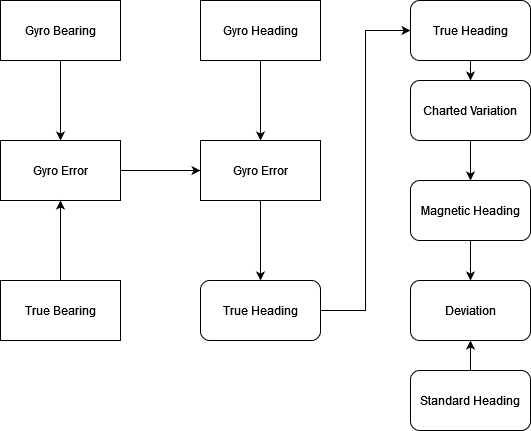
\includegraphics[width=0.8\textwidth]{static/getgettvmdc.drawio.png}
	\caption{A common way to organize the calculations for calculating Gyrocompass Error, Variation and Deviation of the Standard Compass, as required for all watches.}
	\label{fig:getget}
\end{figure}
\clearpage
\subsubsection{Azimuth} \label{doubleget}
It is important to get into a good routine for taking an Azimuth on your bridge watch.
The CWO is required to complete one on all watches on the Bear, and azimuths are some of the only practical industry celestial.
You are required to log information in the Ship's Log and the Compass Observation book.
The Ship's log wants the gyro course, standard course, GE, VAR, and DEV, True Heading, and the CWO's signature.
The Compass record book wants time, date, Lat, Lon, gyro CSE, standard CSE, gyro bearing, true bearing, GE, VAR, and DEV, True Heading, repeater used, and the CWO's initials.
To successfully complete your azimuth, you need 4 pieces of information simultaneously.
\begin{enumerate}
	\item Ship's Position
	\item Time (UT and LT) of Observation
	\item Observed Bearing
	\item Ship's Heading (Steering and Checking)
\end{enumerate}
Information on the ship's heading can always be had by asking the helmsman what they are steering and checking, and if they are any good they will still be on mostly the same course when you ask as when you were when you made the observation.
You may ask your BTM to record the Ship's Position off the GPS at the moment you take your observation, but if you do that, he can't be standing next to your to hold your wristwatch.
At the very least, you have to make the shot yourself.
If you know the ECDIS logbook frequency, you can kill birds 1 and 2 (and half of bird 4) by timing your shot to land on a time that the ECDIS records information, like at the top of the hour, as that ECDIS log entry will have Lat, Lon, Gyro Head, and (zone and Greenwich) time.
You still must observe your shot and ask the helmsman what she is checking.
As far as calculating GE and DEV, consider the format in Figure \ref{fig:getget}.
Fill in the steering and checking headings as reported by the helmsman, the observed gyro bearing you saw, and the variation off the chart.
Use the \ref{eq:Z} Equation to get Azimuth Angle, convert to true bearing, and find the Gyro Error.
Apply the Gyro Error to the Gyro Heading to get True Course. 
True Course \textsuperscript{+W}\textsubscript{-E} Variation = Magnetic Heading, and the difference between magnetic and standard headings is the deviation.
\subsubsection{Fix}
The important thing to note about taking Celestial Fixes on your navigational watch is the use of the communal plotting sheet.
This is in some ways easier, because you no longer have to set up your longitude lines on your own and you have a trackline.
On the other hand, you must share this chart and you cannot take it to the nav lab to submit for your credit.
To submit a fix, take a photograph of the plotting sheet and submit your work separately with a note to see the photo you will provide the instructor.
When making your fix, you may initial the lines of position that you have constructed, as well as the running fix if it is on your watch.
This note is the most important when daytime running fixes of the Sun are required.
The BTM of the 08-12 watch creates an LOP from the sun at 0903, marks the AP and leaves a dashed construction line to the LOP, initials the LOP, and also creates an 0903 DR.
You are the CWO of the 12-16 watch, you observe LAN at 1222, and a post meridian LOP \astrosun{} at 1541. 
\begin{enumerate}
	\item Make 1222 and 1541 DR
	\item Draw 1222 LAN Lat and sign
	\item Place 1541 AP, dashed construction line, and 1541 LOP and sign
	\item Decide what time you want the fix to reflect, (I would recommend 1600 in this case, to provide the oncoming bridge watch the most up to date position information)
	\item Advance/Retard AM and PM APs to the desired fix time, and move the 1222 LAN Lat LOP directly
	\item Enclose and sign the running fix
	\item Take a picture.
\end{enumerate}

An important aspect of the morning or evening fix of the stars is not neglecting your watch duties.
An experienced navigator can spend 6 minutes finding and shooting the stars, and then 5 minutes each converting that information into LOPs, and a final 2 minutes each plotting them. 
However, even though I am fast enough to spend only 30 minutes shooting, reducing, and plotting a fix, that's a lot of time not spent doing your mandatory duties, maintaining a good lookout, and standing a good watch.
Take care to not spend long with your nose in the book.
Take a sight, back to watch, sight, watch, sight, watch, calculate, watch, calculate, watch, calculate, watch, plot, watch, plot, watch, plot, enclose and sign, watch.
On my cruise the 04-08/16-20 LWO was very strict about this.
Delegate what you can to your BTM.
\clearpage
\printbibliography
\end{document}
